\documentclass[dvipdfmx, 9pt, a4paper]{jsarticle}
\usepackage[margin=15mm]{geometry}
\usepackage{fancyhdr}
\usepackage{multirow}
\usepackage{amsmath,  amssymb}
\usepackage{type1cm}
\usepackage{latexsym}
\usepackage{algorithmic}
\usepackage{algorithm}
\usepackage{ascmac}
\usepackage{braket}
\usepackage{listings,jvlisting}
\usepackage{tcolorbox}
\usepackage[utf8]{inputenc}
\usepackage{color}

\renewcommand{\theequation}{\arabic{section}.\arabic{equation}}
\renewcommand{\thefigure}{\arabic{section}.\arabic{figure}}
\renewcommand{\thetable}{\arabic{section}.\arabic{table}}
\makeatletter
\@addtoreset{equation}{section}
\@addtoreset{figure}{section}
\@addtoreset{table}{section}
\AtBeginDocument{
  \renewcommand*{\thelstlisting}{\arabic{section}.\arabic{lstlisting}}%
  \@addtoreset{lstlisting}{section}
}


\numberwithin{equation}{section}

\DeclareFixedFont{\ttb}{T1}{txtt}{bx}{n}{9}
\DeclareFixedFont{\ttm}{T1}{txtt}{m}{n}{9}
\definecolor{deepblue}{rgb}{0,0,0.5}
\definecolor{deepred}{rgb}{0.6,0,0}
\definecolor{deepgreen}{rgb}{0,0.5,0}

\renewcommand{\baselinestretch}{0.78}
\newcommand{\bm}[1]{{\mbox{\boldmath $#1$}}}
\newcommand{\bnabla}{\bm \nabla}
\newtheorem{Proof}{証明}
\def\qed{\hfill $\Box$}

\newcommand\pythonstyle{\lstset{
language=Python,
basicstyle=\ttm,
morekeywords={self},
keywordstyle=\ttb\color{deepblue},
emph={MyClass,__init__},
emphstyle=\ttb\color{deepred},
stringstyle=\color{deepgreen},
frame=tb,
showstringspaces=false
}}

\lstnewenvironment{python}[1][]
{
\pythonstyle
\lstset{#1}
}
{}

\newcommand\pythonexternal[2][]{{
\pythonstyle
\lstinputlisting[#1]{#2}}}
\newcommand\pythoninline[1]{{\pythonstyle\lstinline!#1!}}

\begin{document}
\begin{center}
{\fontsize{18pt}{1pt}\selectfont 強化学習}\\
\end{center}
\section{強化学習問題}
学習という意味を考えたとき、恐らく自転車の乗り方を覚えたときのような試行錯誤による学習と、授業を通して知識を得る学習の2つを思い浮かべる。確かにどちらも学習と言えるが、教師的な存在の有無という点で両者は異なる。{\bf 強化学習}は前者的な学習を指し、後者は教師あり学習に分類される。\par
強化学習を一言で表すならば、{\bf エージェント}が{\bf 環境}から{\bf 報酬}信号を受け、それを基に何をすべきか学習する仕組み」である。強化学習ではエージェントや環境、並びに報酬と言う言葉をよく用いる。エージェントとは学習や行動を担うものであり、ロボットや制御器が該当する。環境はそっくりそのままエージェントが置かれた環境のことであるが、実空間の環境だけでなく例えば将棋ゲームといったものも含まれる分、私たちが普段使う環境よりも広い意味を持つ。\par
エージェントや環境と比べ、報酬は強化学習の中でより特徴的な存在だと言える。まず、強化学習が教師あり学習と最も異なる点は、行動の評価を基に学習することである。つまり、教師あり学習では最適な行動を直接教えて貰うのに対し、強化学習では行動の良し悪しを教えて貰えるものの、最良か否かまでは分からない。この良し悪しに関連する数値が正に報酬である。\par
もう少し強化学習の枠組みを言うなら、エージェントと環境は離散的な時間ステップ$t=0, 1, ...$において相互作用する。各時刻において、エージェントは何かしらの状態$s_t \in \mathcal{S}$($\mathcal{S}$は可能な状態の集合)に置かれ、これに対し何か行動$a_t \in \mathcal{A}(s_t)$($\mathcal{A}(s_t)$は$s_t$状態化で取り得る行動の集合)を取る。その結果、エージェントの状態は$s_{t+1}$に遷移し、フィードバックとして報酬$r_{t+1}$を受け取る。エージェントは一連の報酬$r_t(t=1, 2, ....)$を受け取って、今までの行動$a_t(t=0, 1, ....)$を改める(学習する)。以上の枠組みを図式化したものが図1.1である。\par
強化学習の問題では不確実性が随所に現れる。例えば状態遷移$s_{t+1}$や受け取る報酬$r_{t+1}$は不確かであることが多い。ちなみに、$s_{t+1}$に関する確率分布が$s_t$と$a_t$のみに依存し、かつ$r_{t+1}$に関する確率分布が$s_t$と$a_t$と$s_{t+1}$のみに依存する場合、このような強化学習問題を{\bf マルコフ決定過程}({\bf MDP})と言う。従って図1.1の枠組みはMDPについて述べていたのであった。残念なことに、MDPを仮定できない環境も多く存在する(例えばトランプの大富豪。今の持ち札だけでなく、相手の行動履歴からも自分の行動を判断した方がよい)。ただし、そういった問題に取り組むときも、確率過程をシンプルにするために、何とかしてMDPに近似できないか考察すべきである。本資料では全ての環境に対しMDPであることを仮定する。\par

\begin{figure}[b]
\begin{center}
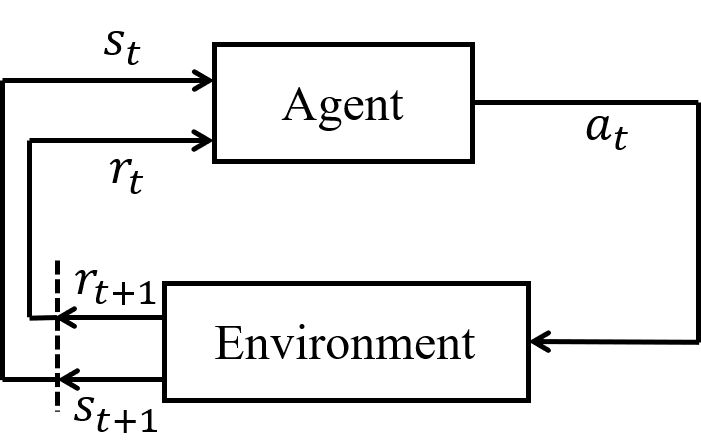
\includegraphics[width=8cm]{fig1_1.png}
\caption{強化学習の概念図。}
\end{center}
\end{figure}

$s_t=s$かつ$a_t=a$のとき、$s_{t+1}=s'$となる確率を$\mathcal{P}^a_{ss'}$と書くことにする。つまり、
\begin{equation}
\mathcal{P}^a_{ss'}\equiv{\rm Pr}\{s_{t+1}=s'|s_t=s,a_t=a\}
\end{equation}
である。このような確率を{\bf 遷移確率}と言う。またこのときの$r_{t+1}$の期待値を$\mathcal{R}^a_{ss'}$と書く。つまり、
\begin{equation}
\mathcal{R}^a_{ss'}\equiv{\rm E}\{r_{t+1}|s_t=s,~a_t=a,~s_{t+1}=s'\}
\end{equation}
である。これは$(s_t,a_t,s_{t+1})$を入力とした関数と見なせるため、{\bf 報酬関数}と呼ぶこともある。\par
強化学習では行動の選択も不確実性を有するものとして扱う。状態$s_t=s$のときに$a_t=a$を選ぶ確率を$\pi(a_t=a|s_t=s)$と書き、$\pi(a_t|s_t)$のことを{\bf 方策}と言う。強化学習の目標は良い方策を得ることであり、学習の間方策は頻繁に修正される。\par
方策に不確実性を与える理由の一つに、探索的な学習の促進がある。前述の通り、強化学習では最良の行動を教えてもらえない。そのため、収益(後述)を多く得られる行動を自ら見つけなければならない。一方で最適な方策は、これまでの学習結果に限って考えれば最適と思われる行動を選択するようなものでなければならない。つまり、学習中の方策にはこれまでの知識の活用と、更に良いと言える行動がないかの探索が求められる。この活用と探索は進化計算における選択と突然変異に似ている。また、方策に不確実性を与えることは明らかに探索的な作用である。もちろん、学習終盤では探索行為を控えなければならない(本来所望していた方策は必ず最適な行動をとるようなものであるため)。活用と探索については後ほどより深く議論する。\par
もう一つ方策に不確実性を与える理由として、不確実な方策自体が最適と言える場合もあることを述べておく。例えばポーカーの問題を考えよう。ポーカーでは相手を惑わすために、ときに不合理な行動を取る。このような高度な技法をエージェントに学ばせるには、不確実性のある方策を考えなければならない。\par
さて、これまでの議論より、行動選択を左右する方策、状態遷移を司る環境、そして報酬が強化学習問題の中核を成すことに気付く。これらの中でエージェントが作用できるのは方策のみである。状態は物理系の状態や将棋の盤面に相当するので、エージェントが決められないのは当然であろう。報酬に関しては、エージェントや環境よりも問題設定者や解析者が決める。エージェントは報酬信号から行動を改めるので、達成したいことに即して私たちが報酬を定義する。

\subsection{収益と価値関数}
\subsubsection{収益}
ここまでエージェントは報酬信号を受け取ることは触れてきたが、具体的にこれをどう活用するのかまでは言及してこなかった。ここで報酬信号とは、時刻$t$のときにそれ以降で受け取る報酬列$r_\tau{\tau=t+1, t+2, ....}$のことである。当然ながら時刻$t$で実施した行動$a_t$は報酬信号に影響を与える。\par
報酬信号が与えられたときに、$a_t$の良否評価の方法は非常に重要である。仮に即時的な報酬のみを考えたならば、$a_t$は$r_{t+1}$の値によってのみ評価される。これは一見良さそうに見えるが、あまり上手くいかないことも多い。\par
例えば私たちの生活の中で、この日は休むという選択を取ったとする。すると体の疲労は取り除かれ、直感的に良い報酬を得られそうである。ただし、この結果から休むという行動が良いと評価するのは安直かもしれない。もしもその日に大学の必修科目のテストがあれば、来年度に留年という結果が待っているだろう。留年の責任は休むという行動が取るべきで、決して留年が決まった直前の行動ではない。このようにエージェントに高度な目標を達成してほしい場合、エージェントは長期的な報酬も含めて行動の評価をしなければならない。そのため報酬信号を全体的に見ることは重要である。\par
これを踏まえたとき、評価指標としてまず初めに思い浮かぶのが、報酬の総和
\begin{equation}
R_t=r_{t+1}+r_{t+2}+....
\end{equation}
であろう。これを{\bf 収益}と言う。ただし、報酬の設定によっては$R_t$は容易に発散する。特に恒常的に動く機械の制御のような問題では、報酬信号は無限に続くので発散しやすい。\par
そこで、{\bf 割引率}$\gamma(0 \leq \gamma \leq 1)$を導入し、式(1.3)を
\begin{equation}
R_t=r_{t+1}+\gamma r_{t+2}+\gamma^2r_{t+3}...=\sum_{k=0}^\infty \gamma^kr_{t+k+1}
\end{equation}
のように修正する。これを{\bf 割引収益}と言う。$\gamma=1$のとき、割引収益は収益と等しくなる。一方で$\gamma=0$のとき$R_t=r_{t+1}$となるので、エージェントは即時的な報酬からのみ学習するようになる。$\gamma$がこれらの間を取る場合、割引収益は時刻$t$に近いときに得た報酬に重みを持たせつつ、報酬信号全体を加味するようになる。

\subsubsection{エピソードタスクと連続タスク}
ところで、エージェントが達成しようとする問題をタスクと呼ぶことがあるが、強化学習のタスクには{\bf エピソードタスク}と{\bf 連続タスク}の2種類がある。\par
エピソードタスクは終端状態という特別な状態を持つ。これは例えばゲームオーバーやゲームクリアによる終了や、組み立てロボットが作業を完了した状態などである。エピソードタスクの場合、式(1.4)のように報酬信号が無限に続くことは稀である。\par
一方で連続タスクは終端状態を持たないタスクのことで、例えばエアコンの温度管理タスクなどが挙げられる。連続タスクの割引収益は式(1.4)の通りである。また、式(1.3)の収益は連続タスクの場合特に発散しやすい。\par
このように、一見するとエピソードタスクと連続タスクで収益の定義を微修正しなければならない気もするが、少しだけエピソードタスクの解釈を拡張すれば、エピソードタスクでも式(1.4)を使うことができる。例えば$t=T$で終端状態に達したとき、本来なら$T+1$以降の報酬はないはずだが、そこを$r_\tau=0(\tau=T+1, T+2, ...)$と拡張する。そうすればエピソードタスクでも式(1.4)を使えるし、割引収益の値も変わらない。本資料では特に断りがない限りこれを前提にして、エピソードタスクと連続タスクを統一的に記述する。
\subsubsection{価値関数}
ところで状態遷移や報酬には不確実性があるので、ある状態のときにある行動を取ったとしても、その後に得られる収益にもバラつきがある。従って、収益を評価指標と述べたが、厳密には「強化学習は期待される収益が最大となるような方策を求める」と言った方が良さそうである。\par
{\bf 価値関数}とは状態(もしくは状態行動対)の関数であり、そこから後に得られる収益の期待値を返す。入力である状態(もしくは状態行動対)から以後の状態遷移と行動選択は方策に依存するため、価値関数も方策に依存する。従って価値関数は方策毎に定義される。\par
状態のみを入力とする価値関数のことを{\bf 状態価値関数}と言い、$V^\pi(s)$と書く。定義より、$V^\pi(s)$は
\begin{equation}
V^\pi(s)={\rm E}_\pi\{R_t|s_t=s\}={\rm E}_\pi\left\{ \sum_{k=0}^\infty \gamma^kr_{t+k+1}|s_t=s \right\}
\end{equation}
となる。ここで${\rm E}_\pi$は方策$\pi$に従ったときの期待値を表す。定義より、終端状態の状態価値関数はゼロとなる。次に、状態と行動を入力とする価値関数のことを{\bf 行動価値関数}と言い、$Q^\pi(s, a)$と書く。定義より、$Q^\pi(s, a)$は
\begin{equation}
Q^\pi(s, a)={\rm E}_\pi\{R_t|s_t=s, a_t=a\}={\rm E}_\pi\left\{ \sum_{k=0}^\infty \gamma^kr_{t+k+1}|s_t=s, a_t=a \right\}
\end{equation}
と書き表される。行動価値関数でも、終端状態での値はゼロとなる。\par
価値関数は経験に基づいて推定することができる。例えば状態価値関数の場合、ある状態$s$から方策に従って行動したときに収益$R_t$を得たとする。これを何度か経験し、アンサンブル平均から$V^\pi(s)$を推定できる。行動価値関数に関しても同様である。後述するモンテカルロ法などは価値関数の推定にこのアプローチを取る。一方で遷移確率と報酬関数が既知である場合は、実際に行動せずとも方策毎に価値関数を推定できる。後述する動的計画法はこのアプローチを取る。

\subsection{Bellman方程式}
\begin{figure}[t]
\begin{center}
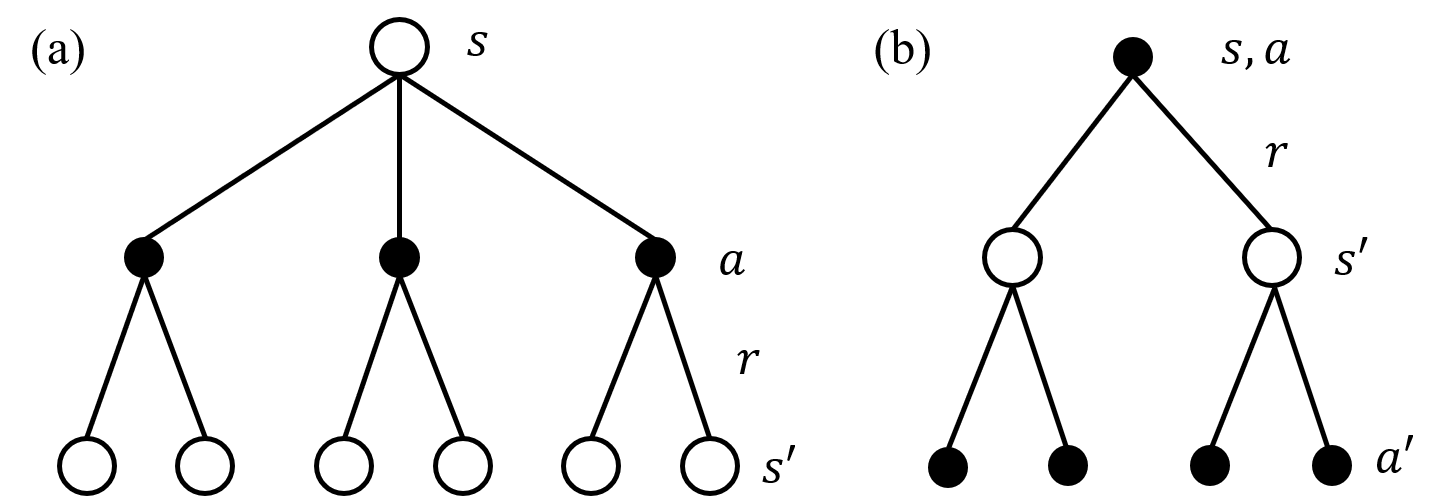
\includegraphics[width=8cm]{fig1_2.png}
\caption{(a)状態価値関数のバックアップ線図(b)行動価値関数のバックアップ線図。}
\end{center}
\end{figure}

本節では価値関数の再帰的構造に着目して、価値関数に関する方程式を導出する。\par
まずは状態価値関数について議論しよう。そこで{\bf バックアップ線図}というものを新たに導入する。図1.2(a)は状態価値関数に関するバックアップ線図である。白いノードは状態を表しており、根の部分の状態$s$が今の状態を表している。$s$と繋がっている黒いノードはそれぞれ一つの行動$a$を表している。方策は確率的性質を持つため、$s$の後に複数の行動$a$が繋がっている次第である。$s$のときに$a$の行動を取ったとき、エージェントは状態$s'$に遷移する。式(1.1)より、状態遷移も不確実性を有するため、$a$の後にいくつかの白いノードが繋がる。$s'$に遷移したとき、環境から報酬$r$を貰う。図1.2のように行動から状態へと繋がるエッジ上に報酬を記載する。\par
ここで状態価値関数の方程式を導出する。状態価値関数は定義より、
\begin{equation}
\begin{array}{ll}
V^\pi(s) & ={\rm E}_\pi\left\{ \sum_{k=0}^\infty \gamma^kr_{t+k+1}|s_t=s \right\} \\
 & ={\rm E}_\pi\left\{ r_{t+1}+\gamma\sum_{k=0}^\infty \gamma^kr_{t+k+2}|s_t=s \right\} \\
 & =\sum_{a \in \mathcal{A}(s)}\pi(a|s)\sum_{s'}\mathcal{P}^a_{ss'}\left[\mathcal{R}^a_{ss'}+\gamma{\rm E}_\pi\left\{ \sum_{k=0}^\infty \gamma^kr_{t+k+2}|s_{t+1}=s' \right\}\right] \\
 & =\sum_{a \in \mathcal{A}(s)}\pi(a|s)\sum_{s'}\mathcal{P}^a_{ss'} \left[\mathcal{R}^a_{ss'}+\gamma V^\pi(s')\right] \notag
\end{array}
\end{equation}
が成立する。この式は重要なので、始めと最後だけを残した方程式を再度記載する。\begin{equation}
V^\pi(s)=\sum_{a \in \mathcal{A}(s)}\pi(a|s)\sum_{s'}\mathcal{P}^a_{ss'} \left[\mathcal{R}^a_{ss'}+\gamma V^\pi(s')\right].
\end{equation}
これを{\bf Bellman方程式}と言う。Bellman方程式の意味は図1.2(a)からよく読み取れる。Bellman方程式は状態の数だけ存在するため、式(1.7)から$V^\pi(s)$に関する連立一次方程式を作ることができる。従って、一般的な連立一次方程式の数値解法で状態価値関数は計算できる。\par
次に行動価値関数について議論する。図1.2(b)は行動価値関数に関するバックアップ線図であり、基本的に図1.2(a)と見方は同じである。ただし、根の部分だけ状態と行動の両方を意味している。これは行動価値関数の定義を考えれば当然であろう。初めに取る行動が確定しているため、$s$と$a$のノードを纏めたと考えてもよい。ただし、以後の行動は方策に従って選択されるので、図1.2(a)のように分岐する。\par
行動価値関数は以下のように書き換えられる。
\begin{equation}
\begin{array}{ll}
Q^\pi(s, a)&={\rm E}_\pi\left\{ \sum_{k=0}^\infty \gamma^kr_{t+k+1}|s_t=s, a_t=a \right\} \\
 & = {\rm E}_\pi\left\{ r_{t+1} + \gamma\sum_{k=0}^\infty \gamma^kr_{t+k+2}|s_t=s, a_t=a \right\} \\
 & = \sum_{s'}\mathcal{P}^a_{ss'}\left[\mathcal{R}^a_{ss'} + \gamma {\rm E}_\pi\left\{ \sum_{k=0}^\infty \gamma^kr_{t+k+2}|s_{t+1}=s' \right\}\right] \\
 & = \sum_{s'}\mathcal{P}^a_{ss'}\left[\mathcal{R}^a_{ss'} + \gamma V^\pi(s')\right]
\end{array}. \notag
\end{equation}
ここで、状態価値関数と行動価値関数には
\begin{equation}
V^\pi(s)=\sum_{a \in \mathcal{A}(s)}\pi(a|s)Q^\pi(s, a)
\end{equation}
の関係があるため、最終的に
\begin{equation}
Q^\pi(s, a)=\sum_{s'}\mathcal{P}^a_{ss'}\left[\mathcal{R}^a_{ss'} + \gamma \sum_{a' \in \mathcal{A}(s')}\pi(a'|s')Q^\pi(s', a')\right]
\end{equation}
の方程式を得る。これが行動価値関数に対するBellman方程式である。

\subsubsection{Bellman最適方程式}
これまで強化学習問題の定義と定式化を議論した。特に強化学習は期待収益が最大となるような方策を求めるという視点は重要である。また、収益の期待値として価値関数があり、価値関数はBellman方程式に従うことも紹介した。\par
全ての状態$S$に対して$V^\pi(s) \geq V^{\pi'}(s)$であるならば、$\pi$は$\pi'$よりも優れていると言える(行動価値関数に関しても同様)。実際に強化学習では方策をこのように比較する。他のどれよりも同じか優れている方策を{\bf 最適方策}という。最適方策は少なくとも一つ存在することが分かっており、複数存在することもある。方策比較の定義より、最適方策群$\pi^*$(全ての最適方策を同じ$\pi^*$で表している)は同じ価値関数を共有する。最適方策における状態価値関数$V^*(s)$のことを{\bf 最適状態価値関数}と言う。同様に最適方策における行動価値関数のことを{\bf 最適行動価値関数}と言う。両者は
\begin{equation}
V^*(s)={\rm max}_\pi V^\pi(s),~~~Q^*(s, a)={\rm max}_\pi Q^\pi(s, a) \notag
\end{equation}
の等式を満たす。\par
最適方策の場合、Bellman方程式を違った形で書くことができる。まず、式(1.8)より最適方策についても$V^*(s)=\sum \pi^*(a|s)Q^*(s, a)$が成立する。$V^*(s)$が最大であるということは、方策$\pi^*(a|s)$は$s$が固定された中で$Q^*(s, a)$が最大となる$a$を確実に選択するようなものでなければならない。つまり、
\begin{equation}
\pi^*(a|s)=
\left\{
\begin{array}{ll}
1 & (a = {\rm argmax}_aQ^*(s, a)) \\
0 & ({\rm otherwise})
\end{array}\right.
\end{equation}
だと分かる。このとき$V^*(s)={\rm max}_aQ^*(s, a)$と書ける訳で、ここから更に
\begin{equation}
V^*(s)={\rm max}_a\sum_{s'}\mathcal{P}^a_{ss'}\left[ \mathcal{R}^a_{ss'}+\gamma V^*(s') \right]
\end{equation}
なる関係を導出することができる。これを最適状態価値関数の{\bf Bellman最適方程式}と言う。最適行動価値関数に関しても同様で、
\begin{equation}
Q^*(s, a)=\sum_{s'}\mathcal{P}^a_{ss'}\left[ \mathcal{R}^a_{ss'}+\gamma {\rm max}_{a'}Q^*(s', a') \right]
\end{equation}
なる関係が得られる。\par
状態の数が$N$であるとき、Bellman最適方程式も$N$個存在する。従って、適当な非線型連立方程式の数値解法を用いれば最適価値関数は求まる。また、式(1.12)より最適方策も同時に求まることになる。そのため強化学習問題はBellman最適方程式の数値解析に帰着させることも可能であろう。


\end{document}






\section{動的計画法}
前章でBellman最適方程式を解けば最適方策が求まることを述べたが、実際にそれを解くことは稀である。その理由は沢山あるが、本章に関連するものとして連立方程式の規模の大きさが挙げられる。\par
状態の数が$N$のとき、Bellman最適方程式も$N$個だけ存在することは既に紹介した。現実の多くの問題では$N$の値は非常に大きく、大規模な連立方程式となってしまう。そのため、連立一次方程式の直接法でも見られるように、Bellman最適方程式の数値解法は計算コストが非常に高い。連立一次方程式の場合、計算コストの問題を克服するために反復法が提案された。本章で紹介する{\bf 動的計画法}({\bf DP})は、この反復法に相当する(反復法も計算コストが高いと考えるのが一般的だが、あくまで直接法と比較して低いことに価値を感じてほしい)。\par
ちなみに、Bellman最適方程式の求解が難しい理由として、環境の完全な理解を前提としていることも挙げられる。Bellman最適方程式は$\mathcal{P}^s_{ss'}$が既知でなければ解けない。これは状態$s$のときに$a$の行動を取った場合、$s'$に遷移する確率が完璧に解っていることを意味している。問題によってはそれもあり得るが、あり得ない場合はBellman方程式は原理的に解けない。\par
残念ながらDPも$\mathcal{P}^s_{ss'}$が既知であることを仮定している。それゆえDPも実問題であまり利用されない。しかしながら、DPの議論で扱われる内容は強化学習の根幹を成しているとも言え、学ぶことの意義は深い。\par
DPは更に幾つかの手法で細分化できるが、本資料では{\bf 方策反復法}と{\bf 価値反復法}を紹介する。
\subsection{方策反復法}
方策反復法とは{\bf 方策評価}と{\bf 方策改善}を交互に繰り返し、最終的に最適価値関数や最適方策を得る手法である。\par
方策評価とは、暫定的な方策$\pi$の元でBellman方程式(1.7)を解き、$V^\pi(s)$を得る処理のことである。式(1.8)は連立一次方程式であるため、既存の数値解法が適用できる。一般的にヤコビ法を使うことが多い。\par
一方の方策改善とは、方策評価で得た$V^\pi(s)$に対し、
\begin{equation}
\pi'(a|s)=\left\{
\begin{array}{ll}
1 & \left(a={\rm argmax}_aQ^\pi(s, a)={\rm argmax}_a\sum_s'\mathcal{P}^a_{ss'}\left[\mathcal{R}^a_{ss'}+\gamma V^\pi(s')\right]\right) \\
0 & ({\rm otherwise})
\end{array}\right.
\end{equation}
となるようなグリーディ方策を定め、$\pi$を$\pi'$に置き換える処理のことである。\par
方策評価と方策改善を繰り返すことで、最終的に最適価値関数と最適方策を得る。厳密な証明はしないが、方策反復が収束したということは、状態価値関数は方策と整合性の取れた値になっており、方策は状態価値関数に対してグリーディとなっていることになる。これはBellman最適方程式を満たしており、正に欲しかった最適状態価値関数や最適方策であることを意味する。\par
なお、式(2.1)において行動価値関数が最大となる$a$が複数存在する場合、無理に一つの行動に絞る必要はない。一つの案として、各行動を等確率に選択する方策が考えられる。

\subsection{価値反復法}
方策反復の欠点として、方策評価の反復計算が挙げられる。復習になるが、方策反復法では固定された方策に対して方策評価を行い、その後で更新された状態価値関数からグリーディな方策に更新する。例えば方策評価に$N$回の反復計算を要したとする。そして、実際の方策反復では行わないが、各ステップ毎にグリーディな方策を確認する思考実験を行ってみる。問題によっては$n(<N)$回の時点でグリーディ方策の更新が止まっていることもあるだろう。つまり、各状態間に対する状態価値関数の大小関係は$n$回以降不変であるにも関わらず、状態価値関数の値が更新されるがゆえに、$N$回の反復をしている訳である。これは反復計算時に固定された方策が最適方策であるならば、最適状態価値関数が知れるという意味で有意義かもしれない。しかしながら、結局あとで方策改善があるのなら、グリーディ方策が更新されなくなった時点で方策評価も止めた方がよい。\par
ところで、よく考えてみれば、最適状態価値関数はBellman最適方程式を満たすため、状態価値関数も式(1.11)とヤコビ法の進め方に倣って更新すればよいと気付く。これは前ステップでの状態価値関数と整合したグリーディ方策に対し、状態価値関数を更新するという点で方策反復と同様だが、反復計算の度にグリーディ方策が変わっているため、方策評価における反復計算は1回だけと解釈できる。つまり、先程述べた欠点は克服されている訳である。このような手法を価値反復法と言う。\par
価値反復法であっても、状態価値関数が収束したときはBellman最適方程式を満たしているので、最適状態価値関数が求まることは保証されている。\par
ちなみに、方策反復法のように状態価値関数が収束するまで反復を繰り返す方法や、価値関数のように反復計算を1回で済ます方法以外にも、その間の反復数の解法でも所望の回は求まる。反復数の違う解法は{\bf 一般化方策反復法}と纏めて呼ばれることもある。

\section{エージェントの探査}
前章ではDPによる最適方策の求解を紹介した。Bellman方程式が価値関数の連立方程式と見なせるならば、DPは実用的な手法と成り得る。ただし、DPを利用するならば、遷移確率と報酬関数は既知でなければならない。これは環境に関して完全に理解していることを意味するので、かなり厳しい要求と言える。\par
環境を完全に理解できていない問題に対して価値関数を推定したいならば、DP以外の手法を取らなければならない。そこで1.1.3項で言及したように、エージェントが実際に行動し、収益のアンサンブル平均から価値関数を推定することを考える。方策を固定した中、様々な状態(もしくは状態行動対)に対して十分に標本が得られたならば、そのアンサンブル平均は価値関数のよい推定値となる。\par
アンサンブル平均により価値関数の推定値が得られたら、それを基にグリーディ方策を定めればよい気がするかもしれない。この行為はDPにおける方策改善に相当する。このような進め方はDPのときは上手くいった。\par
しかしながら、エージェントの経験に基づく本アプローチの場合は上手くいかない。2章のグリッド問題を例にして考えてみよう。いま、グリーディではない方策$\pi$に従って、エージェントに複数回行動させ、価値関数の推定に成功したとする。次に得られた価値関数に基づくグリーディな方策に改善する。すると、エージェントはスタート位置から決められた行動しか取らなくなり、いくらタスクを繰り返しても同じ結果しか得られなくなる。状態によってはタスクの中で一度も現れないものもあり、以後標本を集めらない、つまり価値関数の推定ができなくなってしまう。\par
この原因はタスク中に不確実性がなくなったことにある。もちろん強化学習の目標は最適方策を求めることなので、方策のグリーディ化が完全に悪いという訳ではない。極端な例として、全状態を経験するために、完全にランダムな方策のままで価値関数の推定を続けていても、最適方策へと向かう改善は一向に進まない。\par
グリーディ方策に対する対策として、{\bf 開始点探査の仮定}というものがある。これは任意の状態(もしくは状態行動対)からタスクを開始でき、かつそれぞれランダムに選択されるというものである。こうすることで、エージェントは様々な状態(もしくは状態行動対)を経験することができるので、標本収集の問題は解決される。グリッド問題はスタート地点が指定されているものの開始点探査の仮定が成立する例で、適当な状態から初めての収益の計算は可能である。\par
ただし問題によっては開始点探査の仮定は困難であり、特に現実空間を環境にした問題では不可能に近い。例えば歩行ロボットの強化学習の場合、右足を上げた状態や左足が浮く瞬間といったものを初期状態として準備しなければならない。つまり、開始点をそもそも準備するという難しさがあったりする。\par
グリーディ方策に対する別の対策としてあるのが、本章で紹介する{\bf 探査}である。これは暫定的な価値関数に対して、グリーディな行動以外も小さな確率で選択されるような方法である。つまり、グリーディ方策を緩和し、グリーディな行動以外も正の確率を持たせる手法と言える。こうすることで、僅かかもしれないがエージェントは様々な状態(もしくは状態行動対)を経験することができ、引き続き価値関数の推定ができるようになる。\par
DPと違って経験を活用する強化学習の場合、経験と探査のバランスは非常に重要な概念である。学習開始当初の少ない経験しかない中、それを信じ切ってグリーディ方策を設定すれば価値関数の更新は望めない。一方で探査をしすぎると最適方策への収束が困難になる。経験を活かした方策の設定、つまり方策のグリーディ化は前章で既に触れている。本章では残りの探査について議論しよう。

\subsection{バンディット問題}
本章では例題としてバンディット問題を採用する。
\begin{itemize}
\item バンディットには$n$本のレバーがあり、エージェントは1つのレバーを引く。
\item レバーを引くとバンディットから0か1の報酬を得る。どちらが出るかはランダムであり、またその確率もレバーによって変わる。
\item エージェントの目標は、1回のタスクでできるだけ多くの収益を得ることである。
\end{itemize}
バンディット問題はエピソードタスクに分類される。ただし明確な状態というものはなく、レバーを引く前が初期状態$s_s$でレバーを引いた後が終端状態$s_f$と言える。これ以外の状態は存在しないので、$\mathcal{S}=\{s_s, s_f\}$と書ける。行動には$n$通りの選択肢がある。ただし、いずれの行動を選んでも$s_s$から$s_f$に遷移する。つまり、任意の行動$a$に対して$\mathcal{P}^a_{s_ss_f}=1$が成立する。一方で、報酬関数は行動によって異なる。$m$番目のレバーにおいて1の出る確率が$p_m$ならば$\mathcal{R}^m_{s_ss_f}=p_m$となる(ここで$m$は$m$番目のレバーを選択する行動を指す)。\par
以上が本問題の説明である。以後、誤解が生じ得ない限り$s_s$及び$s_f$は省略する。\par
前章では状態価値関数で考えていたが、本問題では行動価値関数$Q(m)$で考える。一般的に環境を完全に理解していない問題では行動価値関数の方が扱いやすい。その理由は単純だが、バンディット問題だとイメージしにくいので、後ほど説明する。式(1.9)より、真の行動価値関数は$Q^*(m)=p_m$となる(バンディット問題の場合、必ず1タイムステップのタスクとなるので、行動価値関数と最適行動価値関数は一致する。そのため真の行動価値関数ならBellman最適方程式を満たすという意味で、$Q^*$の表記を用いた)。ただし$p_m$は未知なので、実際にレバーを何度か引いて推定しなければならない。当然ながら$m$番目のレバーを$M$回引いたとき、各タスクの収益が$\{ x_{m1}, ..., x_{mM}\}$であったならば、行動価値関数$Q(m)$の推定値は$\sum_i x_{mi}/M$となる($\{ x_{m1}, ..., x_{mM}\}$は報酬信号でないことに注意)。エージェントは、探査として様々なレバーを引きつつ、最終的には$p_m$が最大となる行動$m$をできるだけ確実に選択できるようになることを目指せばよい。\par
なお、あるレバーが$k-1$回選択されたときの行動価値関数を$Q_{k-1}$、そのあと更に1回選択されたときの行動価値関数を$Q_{k}$としたとき、両者には
\begin{equation}
Q_{k}=\left(1-\frac{1}{k}\right)Q_{k-1}+\frac{1}{k}r
\end{equation}
なる関係が成立する。ここで$r$は$k$回目の行動で得た報酬である。初期値$Q_0$に関しては本来少し議論しなければならないが、差し当たりゼロとする。式(3.1)の更新則は、これまでの収益の標本結果を保存する必要がないことを教えてくれる。これは計算メモリの節約に繋がるので、強化学習ではこのような更新則を積極的に活用する。

\subsection{$\epsilon$-グリーディ法}
{\bf $\epsilon$-グリーディ法}とは、グリーディ方策に対して探査の余地を与えた方策に関する手法の一種である。具体的には、グリーディ方策に対し、暫定的に最も行動価値の高い行動を$1-\epsilon$の確率で選択する。ただし、$\epsilon$の確率で全ての行動を一様確率で選択する。従って行動価値関数を$Q(a)$、取り得る行動の数を$A$としたとき、
\begin{equation}
\pi=\left\{
\begin{array}{ll}
1 - \epsilon + \epsilon/A & (a = {\rm argmax}_aQ(a)) \\
\epsilon/A & ({\rm otherwise})
\end{array}\right.
\end{equation}
なる方策を設定する。ここで$\epsilon$はハイパーパラメータであり、これが高いほど探査の圧力が強まる。一方でエピソードを重ねるにつれ探査の必要性が弱まることは想像できるので、$\epsilon$の値を徐々に小さくしていくといった方法も考えられる。\par
図3.1は$\epsilon=0.1,~0.01$におけるバンディット問題の学習結果である。どちらの場合も学習するにつれ正答率が上昇しているが、本問題では$\epsilon=0.1$の方が良い結果となっている。

\begin{figure}[b]
\begin{center}
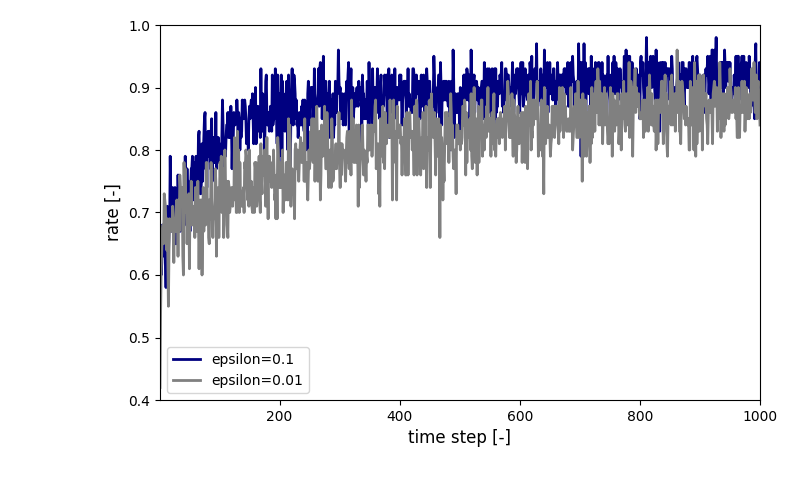
\includegraphics[width=10cm]{fig3_1.png}
\caption{$\epsilon$-グリーディ法によるバンディット問題の学習結果。縦軸は報酬1を得られる確率。}
\end{center}
\end{figure}

\subsection{ソフトマックス行動選択}
$\epsilon$-グリーディ手法は、グリーディでない選択をするときに全ての行動を平等に選択するという特徴を持つ。この特徴はほとんど最悪と思える行動も平等に選択することを許容するため、ときに欠点として扱われる。問題によっては、行動価値に即して行動選択の確率に重みづけをして欲しいこともある。このような選択規則をソフトマックス行動選択規則と言う。\par
ソフトマックス行動選択規則として様々な分布が提案されているが、代表例として
\begin{equation}
\pi(a)=\frac{e^{Q(a)/\tau}}{\sum_b e^{Q(b)/\tau}}
\end{equation}
がある。ここで$\tau$は温度と呼ばれる正の実数である。この分布に従えば、行動価値関数$Q(a)$が高い行動ほど優先的に選択されるようになる。また、選択における不平等さは$\tau$の値を変えることで調整できる。$\tau$を大きくする程$\pi(a)$は一様分布に近づき、$\tau$が低いほどグリーディな選択に近づく。そして$\tau \to 0$の極限では、式(3.3)はグリーディ法と一致する。\par
ソフトマックス行動選択規則の欠点として、$\tau$の設定の難しさが挙げられる。式(3.3)より、知識活用と探査のバランスは$\tau$と行動価値の比率によって決まる。従って前もって行動価値のオーダーが分からない場合、所望のバランスとなる$\tau$の値も決まらない。これに対し$\epsilon$-グリーディ法の$\epsilon$は行動価値関数に依らず決めることができるため、ソフトマックス行動選択規則よりも設定しやすいと言える。そのため、$\epsilon$-グリーディ法とソフトマックス行動選択規則は問題によって使い分けるべきというのが世間の共通認識である。

\subsection{非定常問題}
これまで扱ってきた問題は、各レバーの報酬の確率分布が定常な問題であった。このように環境が定常な問題を定常問題と言う。これに対して、実際の問題では環境が途中で変化するようなこともある。バンディット問題で例えると、各レバーの報酬の確率分布が時々刻々変化するような問題であり、これを非定常問題と言う。\par
式(3.2)の行動価値の場合、各報酬が同じ重み$1/k$で和が取られている。これは、非定常問題問題の場合望ましくない。非定常ゆえに、現時刻よりだいぶ前に得た報酬を今でも得られる保証は無いためである。どちらかというと現時刻に近い頃に得た報酬をより参考にしたいと思うのが普通である。\par
ところで、この$1/k$は学習率(もしくは緩和係数)のような働きをしていることに気付く。また、行動を経験した数に反比例して学習率を下げることで、行動価値関数が収益の期待値となるように制御している。\par
そこで、$1/k$を定数$\alpha(0 \leq \alpha \leq 1)$にしてみよう。すると行動価値関数は
\begin{equation}
Q_k=(1-\alpha)Q_{k-1}+\alpha r=(1-\alpha)^{k}Q_0+\sum_{i=1}^{k}\alpha(1-\alpha)^{k-i}r_i
\end{equation}
に従い更新されていく。ここで$r_i$は行動$a$を$i$回目に取ったときに得た報酬である。式(3.4)の場合、指数関数的に減少する重みが各報酬に掛けられており、直近の報酬ほど大きな重みとなっている。このような行動価値の算出方法を指数加重移動平均と言う。\par
式(3.4)の行動価値関数はもはや収益の期待値とは言えない。ただし、実は定常問題でも有効に働く性質を持っており(後述)、強化学習の分野では式(3.2)より使われている。

\subsection{オプティミスティック初期値}
今まで紹介してきた手法は行動価値の初期値に依存している。例えば指数加重移動平均の場合、初期値はいつまでも行動価値に影響を与える。また、式(3.1)の標本平均による行動価値ならば、一度その行動が取られると初期値に依存しなくなるが、行動がとられるまでは初期値に依存するとも逆に言える。初期値の設定はある意味主観的と言えるので、強化学習において初期値はバイアスと扱われる。\par
ただし、このバイアスは実際のところ問題にならず、むしろ有益な使い方がある。例えば期待収益に関して事前知識がある場合、それを初期値として学習を進める事ができる(これはベイズ統計における事前分布に似ている)。それだけでなく、初期値の与え方によっては学習初期の探査を促すこともできる。\par
例えばこれまでのバンディット問題の場合、各レバーの報酬の期待値は最大でも1であった。そんな中で各レバーの初期値を1以上にしたとする。この時、エージェントはどのレバーを引いたとしてもその結果に落胆し、行動価値の推測値を初期値から下げ、他のレバーへの探査意欲を強める。学習初期はいずれのレバーを引いても結局落胆すると思われるので、当分探査を止めない。このように、探索を促すために与えられた楽観的な初期値のことをオプティミスティック初期値と言う。\par
オプティミスティック初期値の最大の特徴は、$\epsilon=0$のとき、つまりグリーディ法であっても探査できる点にある。ただし、オプティミスティック初期値は学習初期の探査に焦点を当てたものなので、一般の非定常問題には全く役立たない。そのため、オプティミスティック初期値とグリーディ法の組み合わせは危険であり、探査圧力のある手法との組み合わせが求められる。

\section{モンテカルロ法}
前章では探査と方策改善を両立させる手法について議論した。そこで題材としてバンディット問題を採用した理由は、実質的な状態遷移がなく探査行動の考察に集中できると思ったためである。実際の問題では状態遷移があるので、バンディット問題よりも考えることが多い。本章以降はこれまでに学んだ知識を総動員し、3章よりも複雑かつ2章とは違って環境の知識がないような問題に取り組む。そういった問題に対処するための手法は数多く提案されているが、本章で紹介するのは{\bf モンテカルロ法}({\bf MC}法)である。

\subsection{価値関数の推定}
MC法を用いる場合、3章の時と同様エージェントは実際に行動し、エピソードが終了したときの収益を基に価値を推定する。そのため、MC法はエピソードタスクでしか使えない。\par
また、MC法で推定するのは行動価値関数である。これはMC法で状態価値関数を推定してしまうと、方策改善時に多くの計算が必要になるためである。状態価値関数で考えた場合、式(1.11)の右辺が最大となるような行動$a$をグリーディ法に選ぶような方策に改善しようとする。実際DPではそのように改善していたが、これは$\mathcal{P}^a_{ss'}$や$\mathcal{R}^a_{ss'}$について完全に理解していたからこそできた。環境について分かっていない状態だと、式(1.11)の計算にもサンプリングと推定が必要になる。一方で行動価値関数を推定した場合、$Q(s, a)$を最大にする$a$をグリーディに選択するような方策に改善すればよいだけなので、計算コスト的に楽になる。\par
MC法のバックアップ線図を描くならば図4.1のようになる。もちろん方策や状態遷移に不確実性はあるが、行動中のエージェントには分かり得ない。エピソード中に経験した状態と行動、そして途中で得た報酬の記憶のみ有する。また、バックアップ線図の描き方を図1.2(b)のときから変えている。まず、終端の四角は終端状態を表している。加えて状態と行動を一つのペアのような描き方にした。\par

\begin{figure}[t]
\begin{center}
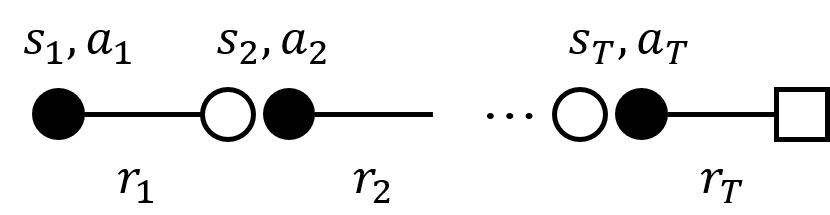
\includegraphics[width=8cm]{fig4_1.png}
\caption{モンテカルロ法におけるバックアップ線図。}
\end{center}
\end{figure}

\subsection{MC法による方策評価}
MC法でもDPと同様に方策評価と方策改善を繰り返すことで最適方策を導き出す。本節では方策評価について議論しよう。図4.1より、状態行動対$(s_1, a_1)$から収益$R_1=\sum_{k=0}^{T-1} \gamma^kr_{k+1}$が得られる(式1.4)。従って$(s_1, a_1)$における行動価値を求めるには、$R_1$の標本平均を計算すればよい。\par
このような考え方だと一つのエピソードからひとつの標本が得られることになるが、実はより効率的に標本を集める方法がある。図4.1を見れば、$R_2=\sum_{k=1}^{T-1} \gamma^kr_{k+1}$は$(s_2, a_2)$の行動価値の標本として利用可能なことに気付く。これは後に続く状態行動対に対しても言えることで、従って一つのエピソードから経験した状態行動対の数だけ行動価値の標本が得られる訳である。\par
もしも一つのエピソード中に同じ状態行動対が複数回現れた場合(例えば図4.1の$(s_1, a_2)$が途中でも現れた場合)、上記に従うとそれに対応する行動価値の標本も複数得られることになる。このような考え方を{\bf 逐一訪問MC法}と言う。一方で、複数回現れた状態行動対のうち、初回の状態行動対についてのみ計算する手法を{\bf 初回訪問MC法}と言う。どちらを用いても、エピソード数が増えるに従い推定値は真の行動価値関数に近づく。一方で、個人的に逐一訪問MC法の方が実装が容易だと考えている。例えば$(s_t, a_t)$以後の収益を$R_t$としたとき、$(s_{t-1},a_{t-1})$の収益は$R_{t-1}=r_{t-1}+\gamma R_t$と求まる。つまり最後の状態行動対から収益を求めることで、無駄な計算を省くことができる。これに対して初回訪問MC法は文字通り初回訪問の状態行動対に対してのみ収益の計算をするので、この計算をしようとしても、いくつか条件分岐を要する。以下は逐一訪問MC法のアルゴリズムである(標本平均では式(3.1)を利用)。
\begin{tcolorbox}[title=逐一訪問MC法における方策評価]
\begin{enumerate}
\item $Q(s, a) = 0$。$n(s, a)=0$。オプティミスティック初期値を使うなら、$Q(s, a)$の初期値はゼロ以外でもよい。
\item 任意の回数$k$だけ以下を繰り返す。
\begin{enumerate}
\item エピソードを一つ生成し、状態行動対$\{(s_t, a_t) | t = [1, T]\}$と報酬$\{r_t|t = [1, T]\}$を保存。
\item $t=T$。
\item $t=1$まで以下を繰り返す。
\begin{enumerate}
\item $n(s_t, a_t) += 1$。
\item $R(s_t, a_t) = r_t + \gamma R(s_{t+1}, a_{t+1})$。ここで$t=T$のときは$R(s_{t+1}, a_{t+1})=0$とする。
\item $Q(s_t, a_t) = Q(s_t, a_t) + \left[R(s_t, a_t) - Q(s_t, a_t)\right]/n(s_t, a_t)$。
\item $t -= 1$。
\end{enumerate}
\end{enumerate}
\end{enumerate}
\end{tcolorbox}

\subsection{方策オン型MC法}
MC法も一般化反復によって最適方策を推定していく。ただし、DPと違って方策評価は収益の標本平均によって行う(4.2節)。そのためエージェントには様々な状態行動対を経験してほしい。本節で紹介する{\bf 方策オン型MC法}は方策改善時に$\epsilon$-グリーディ方策を用いる手法である。別手法である方策オフ型MC法は後述するので、差し当たりオン/オフの意味は考えない。\par
ところでDPの説明の際、方策評価で無限回の反復計算を行わない限り、真の状態価値関数への収束は保証されないことについて言及した。それだけでなく価値反復法のように、状態価値関数値の収束すら要求しない手法も提案されている。これらはMC法でも同様であり、一般的に価値反復法のような考え方でMC法に方策改善は進められる。\par
ただし、2.2節では全ての状態に対し一度だけの更新をしていたのに対し、MC法では一度のエピソードを生成したら直ぐに方策改善に移る点で異なる。つまり前節中アルゴリズムの2.において、$k=1$とする。とはいえそれだと標本数が不十分になるので、アルゴリズムがうまく機能しない。そこで、たとえ方策が変わったとしても、これまでの方策反復中に得た収益$R(s, a)$をすべて保存し、それらの平均をもって行動価値関数を推定することにする。以下は方策オン型MC法のアルゴリズムである。
\begin{tcolorbox}[title=方策オン型MC法]
\begin{enumerate}
\item $Q(s, a)=0$。
\item 任意の回数だけ以下を繰り返し。
\begin{enumerate}
\item エピソードを一つ生成し、状態行動対$\{(s_t, a_t) | t = [1, T]\}$と報酬$\{r_t|t = [1, T]\}$を保存。
\item $t=T$。
\item $t=1$まで以下を繰り返す。
\begin{enumerate}
\item $R(s_t, a_t) = r_t + \gamma R(s_{t+1}, a_{t+1})$。ここで$t=T$のときは$R(s_{t+1}, a_{t+1})=0$とする。
\item $Q(s_t, a_t) = Q(s_t, a_t) + \alpha \left[R(s_t, a_t) - Q(s_t, a_t)\right]$。
\item $t -= 1$。
\end{enumerate}
\item 式(3.2)に従い方策を更新する。
\end{enumerate}
\end{enumerate}
\end{tcolorbox}
行動価値関数は本来$Q^\pi(s, a)$と書かれるように、方策に依存する。そのため、標本の収集中に方策が変わるのは不自然と言える。しかしながら、これでも上手くいくことが経験的に言われており、実用上の問題はないと見なされている。また、上記アルゴリズム中の平均値計算では、標本平均ではなく指数加重移動平均を用いている。これは最近のエピソードの方が方策と整合した収益を出力していると考えられるので、その分重みを持たせるためである。
\subsection{方策オフ型MC法}
前節で方策オン型MC法によるグリッド問題の実装を紹介したが、実はその解法に少しだけ気になる点がある。よく考えてみると、得られた価値関数は$\epsilon$-グリーディ法のようなソフト方策におけるもので、最適価値関数とは乖離している。この乖離は真の価値関数との乖離(2章)とは別の話で、本資料で初めて触れる問題である。\par
DPの場合、方策は常にグリーディだったので、こういった問題はなかった。バンディット問題の場合はソフト方策だが、状態遷移がないおかげでこの問題を考える必要がなかった。例えば、ある状態$s$のときに行動$a$を選択したとする。このとき得られる報酬$r$は方策に依存しない。依存するのは状態遷移後のエピソードなので、それゆえ$(s, a)$に関する収益は方策に依存する。\par
この問題の対処の仕方として二つ考えられる。まず一つ目は無視することである。たとえ最適価値関数が得られなくとも、ある程度グリーディ気味なソフト方策で学習したのならば、得られた価値関数はそこそこ正しく、最終的な方策も有用だと考える。方策オン型MC法はこのような考え方をしている。\par
もう一つの対処の仕方が本節で紹介する方策オフ型MC法である。方策オフ型では、実際に行動する方策({\bf 挙動方策})と、自ら学習し最終的に利用される方策({\bf ターゲット方策})を用意する。挙動方策をソフトにし、さまざまな状態行動対を経験させつつ、ターゲット方策をグリーディなまま学習させていく訳である。そこで、方策オフ型MC法の理解のためにまずは重点サンプリングについて議論したい。
\subsubsection{重点サンプリング}
重点サンプリングとは、ある確率分布の期待値を別の確率分布からサンプリングした結果を用いて推定する手法である。\par
本節では確率分布$\pi(x)$の期待値の計算を考える(ここで期待値を${\rm E}_\pi[x]=\sum \pi(x)x$と考えるが、連続な確率変数ならばこれを積分計算に変えるだけでよい)。定義より、
\begin{equation}
{\rm E}_\pi[x]=\sum \pi(x)x=\sum b(x)\left(\frac{\pi(x)}{b(x)} x\right)={\rm E}_b\left[\frac{\pi(x)}{b(x)} x\right] \notag
\end{equation}
のように書き換えることができる。また、${\rm E}_\pi[x]$の推定値として$\sum x/n$が考えられるので、確率分布$b(x)$に従ってサンプリングしたときは、${\rm E}_\pi[x]$の推定値を$\sum (\pi(x)/b(x))x/n$より計算すればよいことが分かる。これは$b(x)$に対して実現値を$(\pi(x)/b(x))x$と見なしていることに相当する。\par
確率分布$b(x)$の選び方は概ね任意だが、$\pi(x)>0$となる$x$に対して$b(x)>0$でなければならない。さもなければ上式が破綻するためである。一般的に、任意の$x$に対して$b(x)>0$となるような確率分布を設定することが多い。そのため、$b(x)$の分散値は$\pi(x)$と比べて大きくなりがちである。この傾向は$\pi(x)$が(グリーディ方策のように)決定論的な確率分布の場合に色濃く出る。\par
$\rho(x)=\pi(x)/b(x)$としたとき、分散$V_\pi[x]$と$V_b[\rho(x)x]$は
\begin{equation}
V_\pi[x]=E_b[\rho(x)x^2]-\left\{E_b[\rho(x)x]\right\}^2,~~~V_b[\rho(x)x]=E_b[\rho(x)^2x^2]-\left\{E_b[\rho(x)x]\right\}^2 \notag
\end{equation}
となるため、両分散の差は$V_b[\rho(x)x] - V_\pi[x]=E_b[(\rho(x)-1)\rho(x)x^2]$となる。$b(x)$の方が裾野の広い確率分布となっている分、$\rho(x) > 1$となる$x$が大半で、それゆえ重点サンプリング結果の分散値は基のものより高い値となる。これは、サンプリングから期待値を求める際、より多くのサンプル数が必要となることを意味する。強化学習問題によっては$x$の次元数が大きく、かつ多くのサンプルを集められないこともある。このような問題の場合、重点サンプリングの期待値の推定値は大きくずれやすい。この欠点は方策オフ型MC法でも言えることで、大規模な問題ではサンプルの扱いの面で学習に苦労する。
\subsubsection{方策オフ型MC法}
方策オフ型MC法は重点サンプリングを用いて行動価値関数を推定する。ターゲット方策を$\pi(a|s)$、挙動方策を$b(a|s)$とする。一般的に$\pi$はグリーディ方策とし、$b$は$\pi$に対する$\epsilon$-グリーディ方策とすることが多い。\par
方策オン型の場合、$(s, a)$の状態行動対に関する収益$\{R^i(s, a) | i= 1, 2, ...\}$を得たとき、これらの移動加重平均より行動価値関数を推定していた。ここで$R^i(s, a)$は$i$回目に得た$(s, a)$に関する収益である。一方で方策オフ型の場合、$\{\rho^i(s, a)R^i(s, a) | i= 1, 2, ...\}$から行動価値関数を推定する。ここで、$i$回目に$(s, a)$を訪れたのち、${\rm trajectory}^i = \{(s^i_t, a^i_t), (s^i_{t+1}, a^i_{t+1}), ..., (s^i_{T-1}, a^i_{T-1}), (s_T)\}$なる状態遷移を挙動方策は選択したとする($s_T$は終端状態)。このときの$\rho^i(s, a)$は${\rm trajectory}^i$の結果、収益が得られた確率、つまり
\begin{equation}
\rho^i(s, a)=\frac{{\rm Pr}({\rm trajectory}^i|\pi)}{{\rm Pr}({\rm trajectory}^i|b)} \notag
\end{equation}
ということになる。定義より${\rm Pr}({\rm trajectory}|\pi)=\prod \pi(a^i_\tau|s^i_\tau)\mathcal{P}^{a^i_\tau}_{s^i_\tau s^i_{\tau+1}}\mathcal{R}^{a^i_\tau}_{s^i_\tau s^i_{\tau+1}}$であり、${\rm Pr}({\rm trajectory}^i|b)$に関しても同様なので、結局上式は
\begin{equation}
\rho^i(s, a)=\prod \frac{\pi(a^i_\tau|s^i_\tau)}{b(a^i_\tau|s^i_\tau)}
\end{equation}
というように書き換えられる。従って重み$\rho$は状態遷移確率など環境に依存せず、方策にのみ依存する。\par
重みは収益と同様に、最後の状態から巻き戻すようにすれば効率的に計算できる。${\rm trajectory}^i$の場合、$Q(s^i_{T-1}, a^i_{T-1})$に関する重み$\rho^i(s^i_{T-1}, a^i_{T-1})$は1となる。これは、$a^i_{T-1}$の行動を選択することは確定していること、並びにその後すぐ終端状態に到達することから明らかであろう。次に$Q(s^i_{T-2}, a^i_{T-2})$に関する重み$\rho^i(s^i_{T-2}, a^i_{T-2})$は定義より$\pi(a^i_{T-1}|s^i_{T-1})/b(a^i_{T-1}|s^i_{T-1})$となる。同様に、
\begin{equation}
\rho^i(s^i_\tau, a^i_\tau)=\frac{\pi(a^i_{\tau+1}|s^i_{\tau+1})}{b(a^i_{\tau+1}|s^i_{\tau+1})}\rho^i(s^i_{\tau+1}, a^i_{\tau+1})
\end{equation}
より重みを順番に求めていけばよい。\par
また、収益は$R(s_t, a_t)=r_t + \gamma \rho(s_t, a_t) R(s_{t+1}, a_{t+1})$に従い更新していけばよい。なお、初めの行動は方策に依らないので、$r_t$に重みを掛ける必要はない。\par
挙動方策を用いてエピソードを生成し、重みを掛けつつ得られた収益から行動価値関数の推定値を更新する。更に行動価値関数からターゲット方策をグリーディに改善し、それと整合するように挙動方策も改善する。これを繰り返すことで最終的に最適方策を得る。以下は方策オフ型MC法のアルゴリズムである。
\begin{tcolorbox}[title=方策オフ型MC法]
\begin{enumerate}
\item $Q(s, a)=0$。
\item 任意の回数だけ以下を繰り返し。
\begin{enumerate}
\item エピソードを生成し、状態行動対$\{(s_t, a_t)|t=[1, T]\}$と報酬$\{r_t\}$を保存。
\item $t=T$。$\rho=1$。
\item $t=1$まで繰り返す。
\begin{enumerate}
\item $R(s_t, a_t) = r_t + \gamma \rho R(s_{t+1}, a_{t+1})$。ただし$R(s_{T+1}, a_{T+1})=0$。
\item $Q(s_t, a_t)=Q(s_t, a_t) + \alpha[R(s_t, a_t)-Q(s_t, a_t)]$。
\item $t-=1$。
\end{enumerate}
\item 挙動方策$b$を式(3.1)に従い改善する。
\item ターゲット方策をグリーディに改善する。
\end{enumerate}
\end{enumerate}
\end{tcolorbox}


\section{TD法}
MC法は一つのエピソードを生成した後に学習をするのであった。MC法における行動価値関数の更新則は
\begin{equation}
Q_{\pi}(s_t, a_t) \gets Q_\pi(s_t, a_t)+\alpha\left(R_t - Q_\pi(s_t, a_t)\right) \notag
\end{equation}
のように表される。上式から挙げられる欠点として、一つのエピソードが時間的に長い場合、学習を長く待たなければならないことが在る。特に連続タスクの場合はMCを利用することができない(図4.1参照)。このような欠点を克服するために{\bf TD法}が提案された。\par
TD法は行動価値関数を
\begin{equation}
Q_{\pi}(s_t, a_t) \gets Q_\pi(s_t, a_t)+\alpha\left(r_{t+1}+\gamma Q_\pi(s_{t+1}, a_{t+1}) - Q_\pi(s_t, a_t)\right)
\end{equation}
に従い更新していく(一般的にTD法と言うと式(5.1)による更新を指すことが多い。ただし、後に紹介する$n$ステップTD法によれば、式(5.1)は1ステップTD法というTD法の特殊な例である)。つまり、近づこうとする行動価値関数値を$R_t$から$r_{t+1}+\gamma Q_\pi(s_{t+1}, a_{t+1})$に変える訳である。$R_t$は実現値である一方、$r_{t+1}+\gamma Q_\pi(s_{t+1}, a_{t+1})$は$Q_\pi(s_{t+1}, a_{t+1})$を含む分不正確だと言える。ただし、暫定的に$r_{t+1}+\gamma Q_\pi(s_{t+1}, a_{t+1})$は$R_t$の期待値だと言える点で、TD法とMC法は類似する。\par
TD法のバックアップ線図を図5.1に示す。図5.1や式(5.1)からも分かるように、TD法はエピソードを完了することを要求しない。この点でTD法は図1.2(b)で表されるDPに似ている。一方で環境の完全な理解を必要としない点では、MC法と似ている。従ってTD法は「DPのように価値関数の関係式を利用しつつMC法のようにアンサンブルによる価値関数の推定を行う手法」と言える。\par

\begin{figure}[t]
\begin{center}
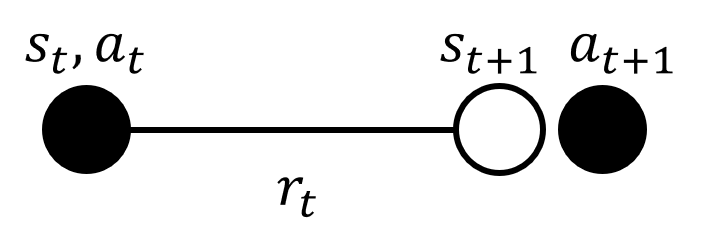
\includegraphics[width=4cm]{fig5_1.png}
\caption{TD法におけるバックアップ線図。}
\end{center}
\end{figure}

理論的に証明されていないが、TD法はMCと比べ、学習における価値関数更新の収束性においても優れていると言われている。この理由は収益のバラつきが小さいためだと直感的に説明されている。いま、話を簡単にするために$Q_\pi(s_t, a_t)$の更新についてのみ考え、それ以外の行動価値関数値は一定であると仮定しよう。MC法の場合は$R_t$、TD法の場合は$r_{t+1}+Q_\pi(s_{t+1}, a_{t+1})$に近づくように更新されていく。このうち$R_t$は$r_{t+1}$や$Q_\pi(s_{t+1}, a_{t+1})$と比べて大きくばらつく($r_{t+1}$が$R_t$よりも小さなバラつきなのは自明。また、状態$s_t$において$a_t$なる行動を取った場合、$s_{t+1}$の取り得る状態の候補は一般的に少ない。従って$Q_\pi(s_{t+1}, a_{t+1})$も$R_t$と比べて小さなバラつきを示す)。従って、TD法における$Q_\pi(s_t, a_t)$の更新の方が安定する。

\subsection{方策オン型TD法(Sarsa)}
方策オン型TD法のことを{\bf Sarsa}と言う。行動価値関数の更新の仕方に違いはあれど、大まかな流れは方策オン型MC法と同様である。以下にSarsaのアルゴリズムを示す。
\begin{tcolorbox}[title=Sarsa]
\begin{enumerate}
\item $Q(s, a)=0$。
\item 任意の回数だけ以下を繰り返し。
\begin{enumerate}
\item $(s,a)$を初期化。
\item 行動$a$を取り、報酬$r$と次状態$s'$を得る。
\item $\epsilon-$グリーディ方策などを用いて、$s'$から行動$a'$を選択。
\item $Q(s, a) \gets Q(s, a)+\alpha(r+\gamma Q(s',a')-Q(s,a))$。
\item $s'$が終端状態の場合は(a)に戻る。それ以外の場合は$s \gets s'$、$a \gets a'$として(b)に戻る。
\end{enumerate}
\end{enumerate}
\end{tcolorbox}

\subsection{方策オフ型TD法(Q学習)}
ここまで本資料を呼んだのであれば、方策オフ型TD法として真っ先に思いつく手法は、4.4節の要領でSarsaを修正したものであろう。つまり、Sarsaに対して挙動方策とターゲット方策を導入し、重点サンプリングを行うような手法である。このような手法は方策オフ型Sarsaと呼ばれる。ただし、方策オフ型TD法として飛びぬけて有名なものにQ学習というものがあり、方策オフ型Sarsaが利用されることは滅多にない。Q学習は重点サンプリングを利用しないし、ターゲット方策も明示的には考えない。特に重点サンプリングを利用しない点は重要で、それによって分散の問題を回避している(4.4.1項)。\par
そもそも、本来所望の最適方策はグリーディ方策なので、$Q_\pi(s_t, a_t)$を$r_t+Q_\pi(s_{t+1}, a_{t+1})$に近づけようとするのではなく、$r_t+{\rm max}Q_\pi(s_{t+1}, a)$に近づけても良さそうである。ここで$\pi$は挙動方策であり、$\epsilon-$グリーディなどに従って行動を選択する。一方で行動価値関数の更新では${\rm max}Q_\pi(s_{t+1}, a)$を考える。これは暗黙的にグリーディなターゲット方策を考えていることに相当する。$Q$学習は方策オフ型の良さを有していることは勿論のこと、計算コストも高くないため、よく利用されている手法である。
\begin{tcolorbox}[title=Q学習]
\begin{enumerate}
\item $Q(s, a)=0$。
\item 任意の回数だけ以下を繰り返し。
\begin{enumerate}
\item $s$を初期化。
\item $\epsilon-$グリーディ方策などを用いて、$s$から行動$a$を選択。
\item 行動$a$を取り、報酬$r$と次状態$s'$を得る。
\item $Q(s, a) \gets Q(s, a)+\alpha(r+\gamma {\rm max}Q_\pi(s_{t+1}, a)-Q(s,a))$。
\item $s'$が終端状態の場合は(a)に戻る。それ以外の場合は$s \gets s'$として(b)に戻る。
\end{enumerate}
\end{enumerate}
\end{tcolorbox}

\section{適合度トレース}
適合度トレースとは強化学習の基本的なメカニズムであり、TD法やMC法をより一般化したものだと言える。適合度トレースによって、これまで分けて考えてきたMC法とTD法を統一的に見ることができ、更に4章や5章で紹介したものよりもより高効率な学習手法を考えることができるようになる。
\subsection{$n$ステップTD法}
適合度トレース説明の前準備として、$n$ステップTD法を議論する。5章で紹介したTD法は式(5.1)のように行動価値関数を更新するのであった。つまり、行動価値関数は行動選択と同じ時間間隔で更新される。\par
一般的に、高度な制御を行うならば時間間隔は短い方が望ましい。一方で行動価値関数の更新に関しては一概にそうとも言えない。あまりにも時間間隔が短ければ$r_{t+1}$が非常に小さな値であり、かつ$Q_\pi(s_t, a_t)$と$Q_\pi(s_{t+1}, a_{t+1})$がほとんど変わらないということが考えられる。この場合、行動価値関数の更新つまり学習は非常にゆっくりとしたものになってしまう。\par
したがって、制御の時間間隔は短いままで、行動価値関数の更新に対してはより長い時間間隔を考えたくなる。これを達成する策は非常に単純で、式(5.1)の代わりに
\begin{equation}
\begin{array}{l}
Q_{\pi}(s_t, a_t) \gets Q_\pi(s_t, a_t)+\alpha\left(R_t^{(n)} - Q_\pi(s_t, a_t)\right) \\
R_t^{(n)}=\sum_{i=1}^n\gamma^{i-1}r_{t+i}+\gamma^nQ_\pi(s_{t+n}, a_{t+n})
\end{array}
\end{equation}
に従って更新すればよいだけである。つまり、$n$ステップ先までは実際に行動し、それ以後の収益に関しては暫定的な行動価値関数値を用いる。このような手法を$n$ステップTD法と言う。また、$R_t^{(n)}$のことを$n$ステップ収益と言う。\par
5章で紹介したTD法は1ステップTD法に相当する。また、MC法は無限回のステップ数のTD法と見なせる(ただし終端状態に到達してからの報酬はゼロで、状態遷移は終端状態で居続けるとする。1.1.2項のエピソードタスクと連続タスクの統一的見方を参照)。従って1以上の有限の整数$n$におけるnステップTD法はTD法とMC法の中間的な手法と言える。

\subsection{TD($\lambda$):前方観測的な見方}
$n$ステップのTD法に対して、問題に合わせて適切な$n$を定めるということはあまりしない。それよりも異なる$n$ステップ収益を平均したのもを利用する(例えば$R_t=(R_t^{(2)}+R_t^{(4)})/4$)。一般的には、ハイパーパラメータ$\lambda(0 \leq \lambda \leq 1)$を用いて、$n$ステップ収益の重み付き平均を
\begin{equation}
R_t^{\lambda}=(1-\lambda)\sum_{n=1}^\infty \lambda^{n-1}R_t^{(n)}
\end{equation}
のように定める。この収益を用いた学習をTD$(\lambda)$と言う。なお、時刻$T$で終端状態に達した場合、それ以後の収益は$R_t$なので、上式を
\begin{equation}
R_t^{\lambda}=(1-\lambda)\sum_{n=1}^{T-t-1} \lambda^{n-1}R_t^{(n)}+\lambda^{T-t-1}R_t
\end{equation}
のように書き表すこともある。\par
前方観測的なTD($\lambda$)は、解釈が容易な一方で効率的なプログラミング実装が難しい。$(s_t, a_t)$における行動価値関数値を更新するために、一つのエピソード実行とそれまでの報酬の保存、並びに各ステップの収益計算が必要になるためである。この問題はMC方がエピソードが長いタスクに利用しにくいことと似ている。そのため、前方観測的なTD($\lambda$)を利用することは滅多にない。

\subsection{TD($\lambda$):後方観測的な見方}
状態行動対$(s_t, a_t)$に達して直ぐに$Q_\pi(s_t, a_t)$を更新できるように修正されたものが、後方観測的なTD($\lambda$)である。一般的にTD($\lambda$)とだけ言うと、後方観測的な見方の方を指す。そのため、以後はTD($\lambda$)と略記する。\par
TD($\lambda$)は各状態行動対に付加的なメモリ変数$e_t(s, a)$を用意する。これを{\bf 適合度トレース}と言う。適合度トレースの初期値$e_0(s, a)$はゼロであり、状態が更新される度に適合度トレースも
\begin{equation}
e_t(s,a)=\left\{
\begin{array}{ll}
\gamma \lambda e_{t-1}(s,a) & ((s,a) \neq (s_t, a_t)) \\
\gamma \lambda e_{t-1}(s,a) + 1 & ((s,a) = (s_t, a_t))
\end{array}
\right.
\end{equation}
に従って更新していく。$\gamma \lambda < 1$であるため、最近訪問された状態の適合度トレースは大きく、訪問後かなり経過した状態の適合度トレースは小さな値となる。以下はSarsaに適合度トレースを加味した学習アルゴリズム(Sarsa($\lambda$))である。
\begin{tcolorbox}[title=Sarsa($\lambda$)]
\begin{enumerate}
\item $Q(s,a)=0$、$e(s,a)=0$。
\item 任意のエピソード回数だけ以下を繰り返す。
\begin{enumerate}
\item $(s,a)$を初期化。
\item 行動$a$を取り、報酬$r$と次状態$s'$を得る。
\item $\epsilon-$グリーディ法などに従い、状態$s'$で取る行動$a'$を選択。
\item $e(s, a) \gets e(s,a)+1$。
\item $\delta = r+\gamma Q(s', a')-Q(s,a)$
\item 全ての$(s, a)$に対して、$Q(s,a) \gets Q(s,a)+\alpha\delta e(s,a)$。
\item 全ての$(s, a)$に対して、$e(s, a) \gets \gamma \lambda e(s,a)$。
\item $s'$が終端状態の場合は全ての$e(s,a)$をゼロに初期化して(a)に戻る。それ以外の場合は$s \gets s'$、$a \gets a'$として(b)に戻る。
\end{enumerate}
\end{enumerate}
\end{tcolorbox}
上記アルゴリズムより、適合度トレースは状態行動対の更新されるべき程度を表していることに気付く。証明はしないが、このアルゴリズムは前方観測的なTD($\lambda$)と同様である。\par
適合度トレースを用いたQ学習も提案されているが、実装コストが高いこと、並びにそれ程効果がないことより、あまり用いられていない。

\section{関数近似による強化学習}
1章から6章の間で強化学習の原理について議論した。MDPのようなモデルを考え、エージェントの学習を方策の最適化と定義した。そして方策の最適化のために価値関数というものを導入し、最適価値関数を見つけるためのアルゴリズムをいくつか紹介した。従ってこれまでの議論によると、私たちは最適価値関数を求めればよいのであった。\par
本章の主題はこれまで深く考えてこなかった$Q(s, a)$の表現の仕方である。そこで改めて前述の行動価値関数更新アルゴリズムを思い出すと(DP、MC、TDのどれでもよい)、行動価値関数の更新は$Q(s, a)$の値の直接的な更新によって成されていることに気付く。つまり、これまでノンパラメトリックな行動価値関数を暗に仮定していた訳である。なお強化学習の分野では、ノンパラメトリックな行動価値関数を用いた場合のことをテーブル形式の強化学習と言う。\par
テーブル形式強化学習において満足のいく行動価値関数を得るには、ときに状態行動対の細かい離散化が必要になる。これは当然ながら計算時間や計算メモリコストの増加を招く。DPの欠点として、十分な離散化による計算時間の増加は既に議論した。これを回避するためにMC法を紹介したが、やはりMC法でもテーブル形式の強化学習だと計算メモリの欠点は回避できない。\par
そこで本章より、真の行動価値関数をパラメトリックな関数で近似することを考える。もしもパラメータの数が状態行動対の個数より圧倒的に少ないならば、上記計算コストの問題を被らない。このような手法を関数近似による強化学習と言う。\par
行動価値関数を$Q(s, a;\bm \omega)$のように表す。ここで$\bm w$は関数$Q$のパラメータである。近似関数自体は線形近似やニューラルネットワーク(NN)など様々である。特にNNを用いた場合を深層強化学習と言う。関数近似による強化学習では、学習によって$Q(s, a)$自体を更新するのではなく、$\bm w$の値を更新する。もしも$Q(s,a;\bm w)$が$\bm w$に対して微分可能であるならば、勾配法による最適化が利用できる。もちろん微分不可能な関数を採用したのであれば、勾配法以外で最適化すればよい。ただし、近年の強化学習の議論はほとんどが深層強化学習であるため、本章も微分可能な関数かつ勾配法による最適化を仮定する。\par
なお、次の章で方策勾配法を紹介するが、これは方策を微分可能な関数で近似する手法である。そのため$Q$を近似する手法と方策勾配法は何れも関数近似による強化学習に分類される。これらを更に明確に分類するために、前者のことを価値ベースの強化学習と一般的に呼ばれている。\par
繰り返しになるが、価値ベースの深層強化学習とテーブル形式の強化学習の間にはノンパラメトリックかパラメトリックかの違いしかない。そのため、テーブル形式の強化学習の資料で紹介したMC法やTD法は価値ベースの深層強化学習でも利用可能である。例えばQ学習は行動価値関数を
\begin{equation}
Q(s, a) \gets Q(s,a) + \alpha\left(r+\gamma {\rm max}_aQ(s_{t+1}, a)-Q(s,a)\right) \notag
\end{equation}
に従い更新するのであった(ここからはパラメータ$\bm w$を省略する)。上式を見たとき、$Q(s,a)$は$r+\gamma {\rm max}_aQ(s_{t+1}, a)$に近づこうとしていることに気付く。従って上式による学習は、$r+\gamma {\rm max}_aQ(s_{t+1}, a)$を是とした$Q$のパラメータ最適化と見なすことができる(もちろんMC法を用いる場合は実際に得た収益$G$を是とした最適化になる。何を是とするかは手法によって変わる)。\par

\begin{figure}[b]
\begin{center}
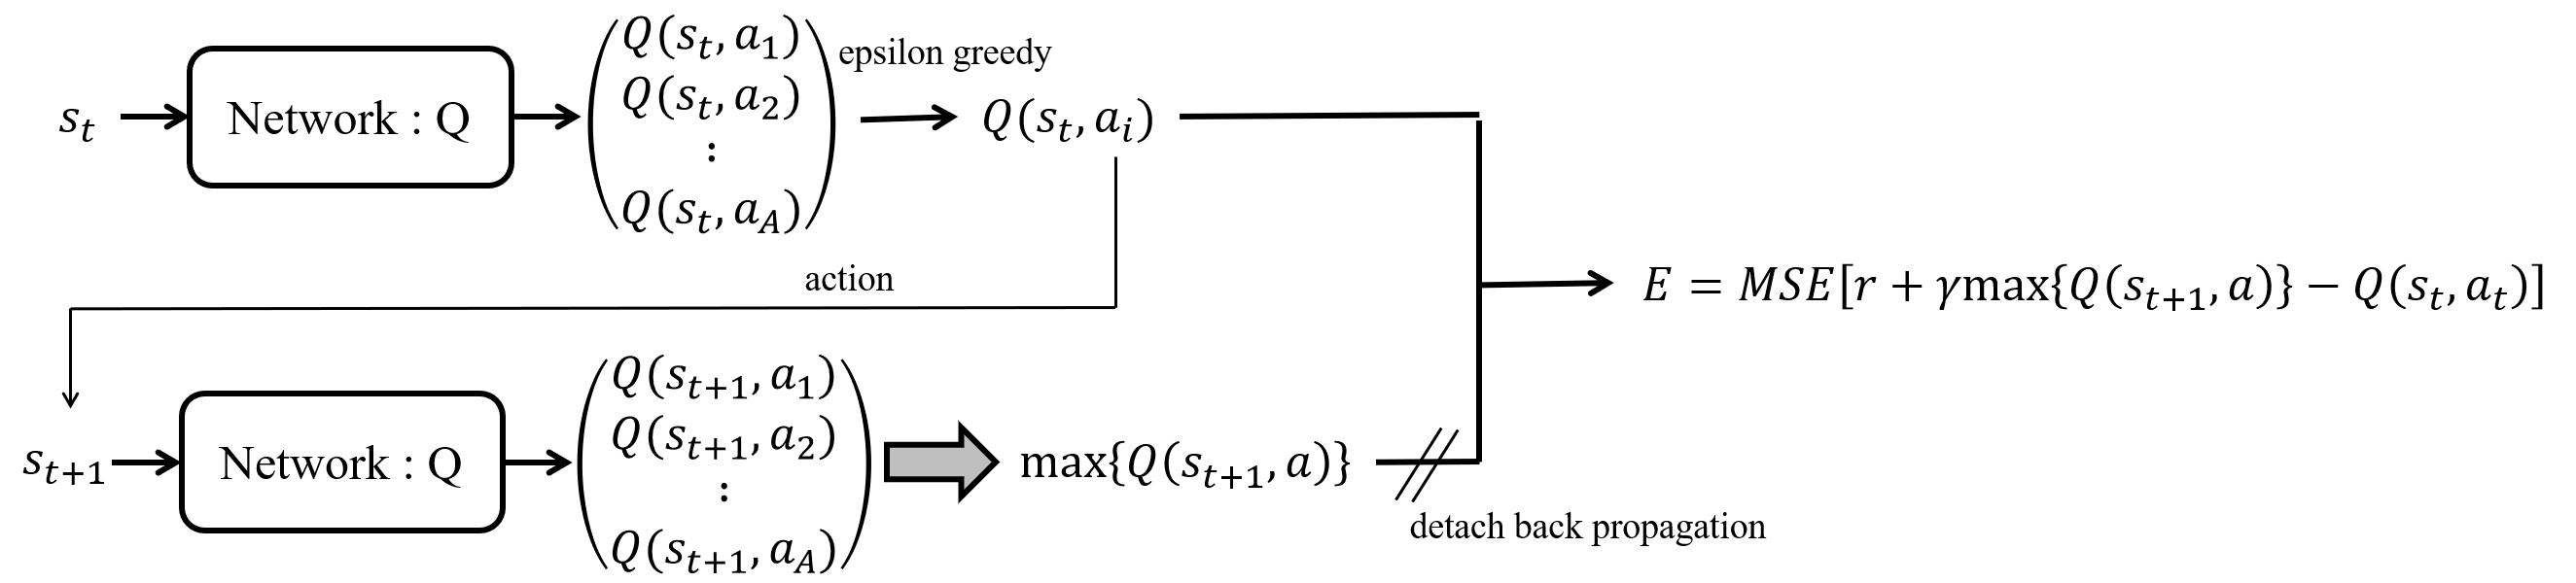
\includegraphics[width=18cm]{fig7_1.png}
\caption{学習の概念図。}
\end{center}
\end{figure}

図7.1にこの学習の概念図を示す(概念図では近似関数をNNとした)。まず、NNの入力は状態ベクトル$s$であり、出力は$Q(s, a)$を行動毎に求めたベクトルである。つまり、取り得る行動の数が$A$である場合、NNの出力は$A$次元ベクトルとなる。$Q(s,a)$という関数の定義を考えれば、状態行動対$(s,a)$を入力とし、$Q(s,a)$を出力とするようなNNを考える方が自然かもしれない。しかしながら、計算コストの都合上このようなネットワークデザインにすることはない。エージェントは行動価値関数値を比較して行動選択することを思い出そう。比較には当然ながら各行動に対する行動価値関数値が必要になる。もしも$(s,a)$を入力とするようなNNであれば、各行動に対する行動価値関数値を計算するのに$A$回の順伝播が必要となる。一方で図7.1のようなNNであれば1回の計算で済むため、計算コストが低い。\par
学習時、NNは状態$s_t$を受け取り、行動価値関数値のベクトル$\bm Q(s_t)$を出力する。ここで$\bm Q(s_t)=(Q(s_t, a_1), ..., Q(s_t, a_A))^{\rm T} \in \mathbb{R}^{A}$である。この推測値を受けてエージェントは、例えば$\epsilon$-グリーディ法などにより行動$a_i$を選択する。その結果状態が$s_{t+1}$を得て、$s_{t+1}$をNNに入力する。得られたベクトル$\bm Q(s_{t+1})$のうち最大値を抽出し、上式に従い誤差$E$を計算する。そして最後に誤差逆伝播を施せば、NNのパラメータが適切に更新される訳である。なお、$Q(s_t, a_t)$が真の値に近づくようにパラメータ更新されるべきなので、${\rm max}Q(s_{t+1}, a)$と$E$は分離されていなければならない。\par
以上が$Q$学習を用いた場合の学習手順である(Q学習以外の場合もほとんど同じ手順に従う)。上式の$\alpha$は深層学習の学習率パラメータにおいて設定すればよい。なお、図7.1の例では誤差関数にMSEを用いたが、これが適切なのかは理論上まだ分かっていない(ただしMSEを用いることが慣習である)。\par
図7.1より、最適値$r+\gamma{\rm max}Q(s_{t+1}, a)$は行動価値関数に依存することに気付く(これはブートストラップを用いる手法全て、つまりMC法以外の全手法に言えることである)。つまり最適値は学習中常に変動する訳であり、一般的な勾配法による最適値問題とは異なる性質を持つと言える。それゆえ強化学習の分野では、前述の最適化手法のことを疑似勾配法と言う。疑似勾配法でも局所的最適値に収束するのかについては、まだ理論的な答えが得られていない。ただし、疑似勾配法だと最適化が難しくなるが、それでも工夫すれば十分に最適解が得られることは経験的に分かっている。\par
価値ベースの深層強化学習の草分け的存在としてDeep Q Network(DQN)が挙げられる。DQNはGoogle DeepMindによって2013年に発表された手法であり、Atariなどにおける高度な制御を披露した。ただし、発表後も改良版が数多く提案されており、今もその流れは止まっていない。具体的な学習技法の紹介は他書に譲る。

\section{方策勾配法}
本章では方策勾配法という強化学習手法を議論する。これまでに紹介した強化学習手法は最適価値関数を学習し、その結果から最適方策を得ていた。これに対して方策勾配法は最適方策関数を直接学習する。\par
例えば方策を$\pi(a|s;\bm w)$の関数で近似したとする(ここで$\bm w$はパラメータ)。この関数は入力として状態ベクトルを受け取り、各行動に対する確率を出力する。従って行動の数が$A$である場合、出力は$A$次元のベクトルとなる。出力は確率分布を表しているため、出力値の総和$\sum_a \pi(a|s)=1$でなければならない($\bm w$は省略した)。この制約は、例えば近似関数にNNを用いた場合、最後の活性化関数にソフトマックス関数を用いれば容易に満足する。\par
このように特に難しさもなく方策の関数を設定できるわけであるが、方策勾配法は近似方策を柔軟に学習できる点で価値ベースの強化学習よりも優れていると言われている。\par
まず、価値ベースの強化学習の場合は探索を保証するために$\epsilon$-グリーディ法などの、全く最適方策の条件を満たさない方策を用いる必要があった。これに対して方策勾配法は学習を進めるにつれ徐々に決定論的な方策に近づけられる。もちろん$\epsilon$-グリーディ法の$\epsilon$を学習経過とともに徐々に減らしたり、ソフトマックス行動選択の温度を徐々に下げたりすることで、価値ベースの強化学習でも決定論的な方策に近づけることができる。しかしながら、これらパラメータのスケジュールを決めることは事前知識無しだと難しい。\par
また、これまで最適方策としてグリーディな方策を考えてきたが、問題によっては決定論的でない方策の方が優れていることもある。例えばポーカーのブラフを考えたとき、相手を惑わすためにあえて不確かさを有する方策を用意することも考えられる。もちろんソフトマックス行動選択に従う価値ベースの強化学習にもこういったことが可能だが、やはり方策勾配法の方が自然に実現できると言える。\par
最後に、方策勾配法は価値ベースの強化学習よりも効率的に学習できると言われている。問題に依っては、価値関数の評価は複雑であっても行動選択は単純であることがある。このとき、方策勾配法は価値関数を考えないので(後に紹介するActor-Critic法などは価値関数も考える)、確かに学習が容易だと想像できる。また、価値ベースの強化学習で$\epsilon$-グリーディ法を用いている場合、ある状態において行動価値関数が最大となる行動が学習中に入れ替わった場合、方策は大きく変わることになる。これによって学習が不安定になることも指摘されている。\par
しかしながら、学習の効率性についての方策勾配法と価値ベース強化学習の優劣は問題に強く依存する。上記の方策勾配法の長所は確かなのだが、別の理由で価値ベースの強化学習を採用した方がよいこともある。

\subsection{方策勾配定理とREINFORCE}
\subsubsection{方策勾配定理}
全ての状態行動対とそれに対応する方策$\pi(a|s;\bm w)$について、何か性能指標$J(\bm w)$を定めたとする。$J$が大きな値を取るほど良い方策であるように$J$を定めたとき、この強化学習問題は$J$の最大化問題と見なすことができる。従って方策が$\bm w$について微分可能である場合、$\bm w$を勾配法で最適化できる。\par
一般的に$J$には収益の期待値が用いられる。つまり、ある方策$\pi(a|s;\bm w)$が所与であるとき、エピソード的タスクにおいて$J(\bm w) = {\rm E}{\tau \sim \pi}[R(\tau)]$のように定義される。ここで$\tau$はエピソードの軌道であり、$R(\tau)$はこのときの収益である。これは、軌道$\tau$が得られる確率を用いて$J(\bm w)=\sum_{\tau} {\rm Pr}\{ \tau \}R(\tau)$のように書くこともできる。いま$J$の勾配が欲しいので、これを微分すると
\begin{equation}
\bnabla J=\bnabla \sum_\tau {\rm Pr}\{ \tau \}R(\tau)=\sum_\tau R(\tau)\bnabla{\rm Pr}(\tau)+{\rm Pr}(\tau)\bnabla R(\tau)=\sum_\tau R(\tau)\bnabla{\rm Pr}(\tau) \notag
\end{equation}
が得られる($R(\tau)$は$\bm w$に依存しないため$\bnabla R(\tau) = \bm 0$)。ここで
\begin{equation}
\bnabla{\rm Pr}(\tau)=\frac{\bnabla{\rm Pr}(\tau)}{{\rm Pr}(\tau)}{\rm Pr}(\tau)={\rm Pr}(\tau)\bnabla {\rm log}{\rm Pr}(\tau) \notag
\end{equation}
であるため(このような変換を${\rm log}$勾配トリックと言う)、$\bnabla J$は
\begin{equation}
\bnabla J=\sum_\tau R(\tau)\bnabla {\rm log}{\rm Pr}(\tau) \notag
\end{equation}
となる。確率${\rm Pr}(\tau)$は
\begin{equation}
{\rm Pr}(\tau)=p(s_0)\pi(a_0|s_0)p(s_1|s_0,a_0)....\pi(a_T|s_T)p(s_{T+1}|s_T,a_T) \notag
\end{equation}
のように書き表すことができる。ここで$p(s_0)$は初期状態が$s_0$となる確率、$p(s_{T+1}|s_T,a_T)$は状態遷移確率である。上式より、$\bnabla {\rm log}{\rm Pr}(\tau)=\sum \bnabla {\rm log}\pi(a_t|s_t)=\sum \bnabla \pi(a_t|s_t)/\pi(a_t|s_t)$となるため、性能指標の勾配は
\begin{equation}
\bnabla J(\bm w)=\sum_\tau R(\tau) \sum_t \frac{\bnabla \pi(a_t|s_t)}{\pi(a_t|s_t)}
\end{equation}
となる。ここまでの議論は方策勾配定理と呼ばれる定理に関するものである。ただし、方策勾配定理はより一般的に議論されたものであり、これを方策勾配定理とは言えない。
\subsubsection{REINFORCE}
上式を用いれば所望の勾配を求められるが、実際は計算コストの都合ゆえに全ての軌道$\tau$を考えることはしない。その代わりエージェントにエピソード$\tau$を生成させて、
\begin{equation}
\bnabla J(\bm w) R(\tau) \sum_t \frac{\bnabla \pi(a_t|s_t)}{\pi(a_t|s_t)} \notag
\end{equation}
によって勾配を計算する(当然ながら、エピソードを多数生成し、上式の勾配を用いてパラメータを逐次的に更新すれば、近似的に式(8.1)と同様の更新が得られる)。学習率を$\alpha$としたとき、本問題は$J$の最大化問題なので、
\begin{equation}
\bm w \gets \bm w + \alpha R(\tau) \sum_t \frac{\bnabla \pi(a_t|s_t)}{\pi(a_t|s_t)} \notag
\end{equation}
のようにパラメータを更新させることが考えられる。\par
上式は、$R(\tau)$が大きいときに、それに関わった状態行動対$(s_t, a_t)$の方策値$\pi(a_t|s_t)$を大きくさせるような更新を意味している。従って上式による更新は妥当だと直感的に分かるだろう。しかしながら、全ての$\pi(a_t|s_t)$に対して同じ重み$R(\tau)$を掛けることには少し疑問が残る。時刻$t$と$t'$間の部分収益を$R_{t:t'}$と表したとき、$\pi(a_t|s_t)$は$R_{0:t-1}$に何ら貢献していないためである。従って実際は上式を
\begin{equation}
\bm w \gets \bm w + \alpha \sum_t R_t\frac{\bnabla \pi(a_t|s_t)}{\pi(a_t|s_t)}
\end{equation}
のように修正して考えることが多い。ここで$R_t$は式(1.4)より得られる。式(8.2)に従ってパラメータを更新する方策勾配法をREINFORCEと言う。

\end{document}









